Neste capítulo apresenta-se os métodos experimentais utilizados para 
quantificação das concentrações de massa total, das espécies químicas e 
do Black Carbon nas amostras. Empregou-se, respectivamente:
análise gravimétrica, fluorescência de raios X (XRF),
Thermal/Optical Transmittance (TOT) e refletância.
Apresenta-se sinteticamente o desenvolvimento teórico de cada método, bem como 
as condições de uso, procedimentos de calibração, cálculo das incertezas, 
vantagens e desvantagens, entre outros.

Para resolução dos modelos receptores, expõe-se também os métodos 
estatísticos Análise de Fatores (AF) e Positive Matrix Factorizarion (PMF) 
usados na identificação dos perfis de fontes. 

Desensolve-se ainda, uma metodologia para estimativa das incertezas
da calibração da XRF e refletância, fundamentais para análises de PMF,
cuja metodologia emprega a ponderação pelas incertezas.

%%%%
\newpage
\section{Amostragem}
% http://maps.google.com/maps/ms?ie=UTF8&hl=en&msa=0&msid=116003586198857296821.00046d7e7367b947abe12&z=12

\begin{figure}[H]
\begin{center}
  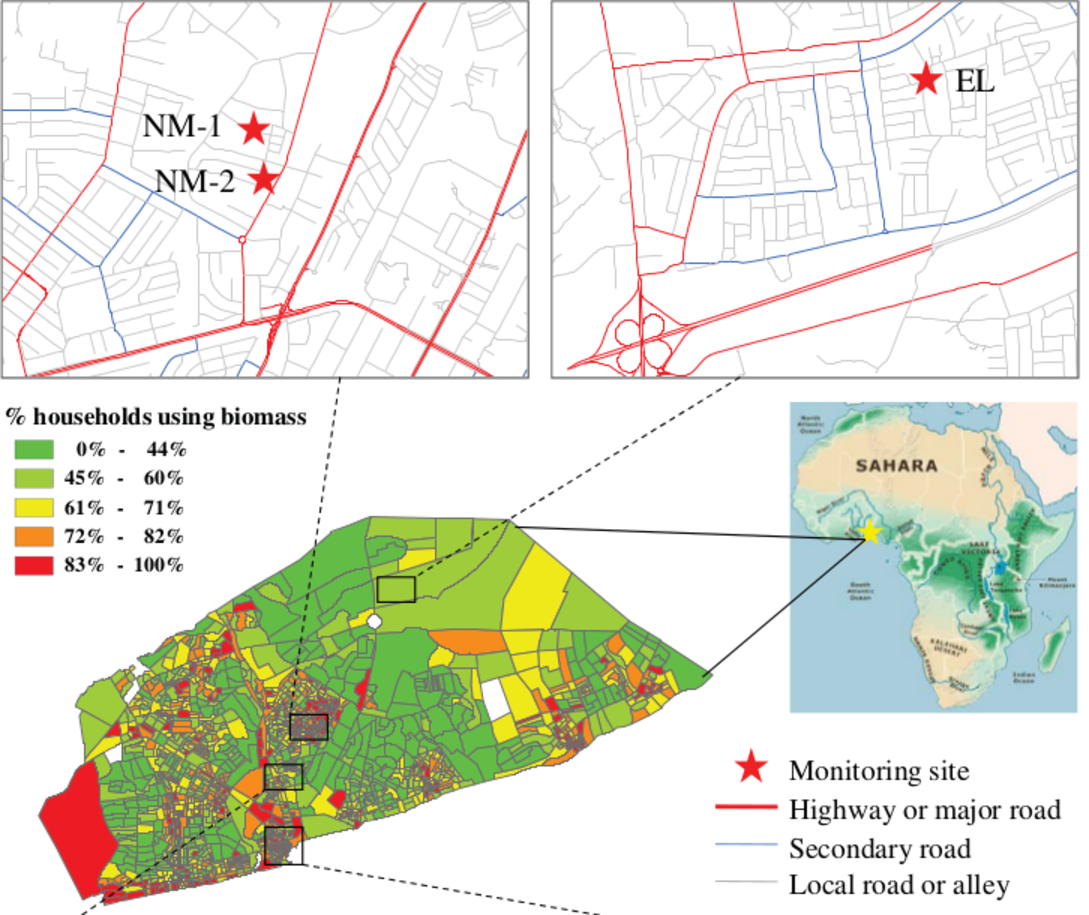
\includegraphics[width=0.6\textwidth]{../inputs/images/zheng/nima_mapa.pdf}
  \caption{Mapa de Nima. NM-1 ponto de amostragem na área residencial e 
           NM-2 ponto de amostragem na avenida. Porcentagem do uso da queima
           de biomassa para preparação de alimentos em residências usando dados
           do censo de 2000 \citep{ghanacensus2003}. Imagem reproduzida do 
           artigo \citet{zhou2013}. \label{fig:nima_mapa}}
\end{center}
\end{figure}

A localização geográfica dos dois pontos de medição, distantes entre si 330
metros, é apresentada na figura
\ref{fig:nima_mapa}, sendo NM-1 na rua \textit{Sam Road}, quarteirão residencial,
e NM-2 na \textit{Nima Road}, via arterial de 2,8 km na direção norte-sul, 
que direciona o tráfego de pequenas vias locais para o centro, atravessando áreas de 
comércios variados. 

A figura \ref{fig:nima_mapa} permite ter uma ideia de duas fontes importantes de 
MP na área de amostragem. Primeiramente, o sistema viário que circunda as 
estações, sendo que boa parte das vias secundárias não são pavimentadas. 
Oferece, ainda, a densidade de uso de biomassa para cozimento de alimentos 
nas residências, baseando-se nos dados do censo de 2000. A tabela 
\ref{table:cookfuel} atualiza genericamente esta informação, considerando o 
censo 2010.

Percebe-se que neste período de 10 anos a fração de uso de gás em Acra 
praticamente dobrou. Saltou de 21,8\% para 41,4\%, enquanto que a soma de carvão
vegetal e biomassa crua reduziu-se em 21\%, mas representando, ainda, 49\% do 
total. Permanece, portanto, sendo o principal combustível utilizado no preparo 
de alimentos.

Aproveitamos aqui para caracterizar também as fontes neste entorno dos pontos de
amostragem, identificados no mapa da figura \ref{fg:acrasources}, o que acreditamos facilitar a posterior discussão dos resultados de modelos receptores.

\begin{figure}[H]
  \centering	
  \includegraphics[width=0.9\textwidth]{../outputs/accra_sources.pdf}
  \caption{Levantamento de algumas fontes poluidora de Acra.
           \label{fg:acrasources}}
\end{figure}

A campanha de coleta ocorreu entre 11 de novembro de 2006 e 15 de agosto de 
2008, com amostragens de 48 horas. O experimento geral tomou 2898 amostras 
($MP_{10}$ e $MP_{2,5}$), em onze sítios localizados em quatro bairros diferentes. 
Deste total, 879 amostras referem-se ao bairro de Nima, tendo sido descartadas 67
devido a comprometimento por avarias como: falta de eletricidade, problemas com 
amostrador, contaminação na manipulação, ausência do operador no horário 
correto das trocas, dentre outros.

%\begin{table}[H]
%  \centering
%    \input{../outputs/samples}
%  \caption{Quantificação total das amostras analisadas no LAPAt porcentagem
%          refletância e XRF-ED \label{table:sampleslogistic}}
%\end{table}

As amostras foram coletadas em filtro de composição de politetrafluoretileno
(PTFE) com diâmetro de 37 mm e 
poros de 0,2 $\mu m$. A área média de deposição, 7,32 ($\pm$ 0,44) $cm^2$, 
foi calculada medindo-se a mancha de deposição com um leitor de espectros 
(nônio de centésimos de mm), sobre 12 filtros amostrados.

Para coleta do MP utilizou-se amostradores Harvard, descritos por 
\citet{marple1987}. Neste equipamento a seleção do diâmetro das partículas 
admitidas no amostrador é feita por impactação inercial. 
Para coleta de $MP_{10}$ o $D_{50}$ do sistema era de 10 $\mu m$, 
com fluxo de 4,0 L/min, enquanto que para $MP_{2,5}$ o $D_{50}$ 
era de 2,5 $\mu m$, com fluxo de 5,0 L/min, medido com 10\% de precisão. 

Filtros brancos de campo e de laboratórios foram separados para avaliar 
possíveis contaminações de fábrica ou de manipulação das amostras. 

Os filtros foram pesados no laboratório da HSPH em balança
microanalítica (Mettler Toledo MT5) com precisão de $\pm 1 \mu g$, 
e ambiente controlado [umidade ($39 \pm 2 \%$), 
temperatura ($20,5 \pm 0,2 ^{\circ} C$) e eliminação de cargas eletrostáticas 
com fonte de polônio]. Os filtros permaneciam ao menos 24 h na sala, 
antes da pesagem, calculando-se a média de duas pesagens que não diferissem 
por mais que 5 $\mu g$.

\begin{table}[H]
	\centering
	\begin{tabular}{llrlr}
  \hline
  \multicolumn{1}{c}{Tipo da} & \multicolumn{2}{c}{Gana (todo país)} & \multicolumn{2}{c}{Acra}                                                           \\
  \multicolumn{1}{c}{fonte de energia} & 2000 & 2010 &  2000 & 2010  \\ 
 \hline & \multicolumn{4}{c}{\% de uso} \\ 
  \hline
  não cozinha           & 3,5 & 5,60 & 4,8 & 6,90 \\ 
\textcolor{red}{biomassa}              & \textcolor{red}{55,8} & \textcolor{red}{40,20} & \textcolor{red}{8,8} & \textcolor{red}{3,50} \\ 
\textcolor{blue}{gás}& \textcolor{blue}{6,2} & \textcolor{blue}{18,20} & \textcolor{blue}{21,8} & \textcolor{blue}{41,40} \\ 
  eletricidade          & 1,1 & 0,50 & 2,2 & 0,90 \\ 
  querosene             & 2 & 0,50 & 4,3 & 1,10 \\ 
 \textcolor{red}{carvão} & \textcolor{red}{30} & \textcolor{red}{33,70} & \textcolor{red}{57,3} & \textcolor{red}{45,40} \\ 
  resíduo de plantação  & * & 0,80 & * & 0,10 \\ 
  pó de serra           & * & 0,10 & * & 0,30 \\ 
  esterco               & * & 0,00 & * & 0,10 \\ 
  outros                & 1,1 & 0,10 & 0,8 & 0,30 \\ 
  \hline
\end{tabular}


	\caption{Percentual relativo dos tipos de fontes de energia usadas para preparação 
		    de alimentos em Gana \citeyearpar{ghanacensus2013}. 
		\label{table:cookfuel}}
\end{table}
